

\tikzset{every picture/.style={line width=0.75pt}} %set default line width to 0.75pt        

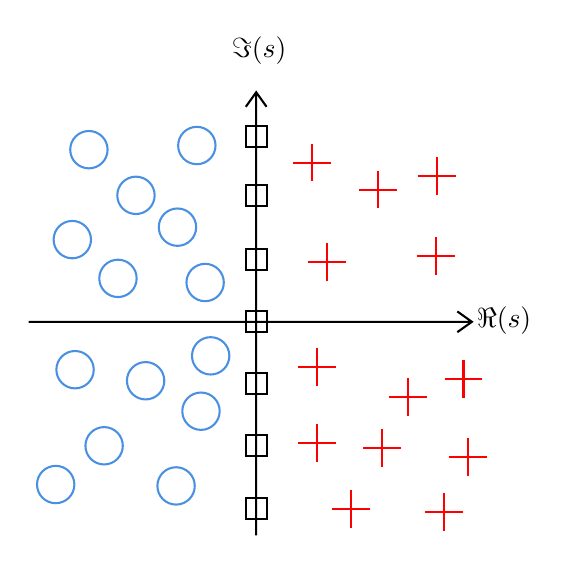
\begin{tikzpicture}[x=0.75pt,y=0.75pt,yscale=-1,xscale=1]
%uncomment if require: \path (0,300); %set diagram left start at 0, and has height of 300

%Shape: Axis 2D [id:dp27678030181731494] 
\draw  (40,160.6) -- (253.5,160.6)(149.6,50) -- (149.6,263.5) (246.5,155.6) -- (253.5,160.6) -- (246.5,165.6) (144.6,57) -- (149.6,50) -- (154.6,57)  ;
%Shape: Square [id:dp29640104318485094] 
\draw   (144.6,155.6) -- (154.6,155.6) -- (154.6,165.6) -- (144.6,165.6) -- cycle ;
%Shape: Square [id:dp5015049228757054] 
\draw   (144.6,125.7) -- (154.6,125.7) -- (154.6,135.7) -- (144.6,135.7) -- cycle ;
%Shape: Square [id:dp5724308304859749] 
\draw   (144.6,94.7) -- (154.6,94.7) -- (154.6,104.7) -- (144.6,104.7) -- cycle ;
%Shape: Square [id:dp8722658997981245] 
\draw   (144.6,66.2) -- (154.6,66.2) -- (154.6,76.2) -- (144.6,76.2) -- cycle ;
%Shape: Square [id:dp035501458242915174] 
\draw   (144.6,185.2) -- (154.6,185.2) -- (154.6,195.2) -- (144.6,195.2) -- cycle ;
%Shape: Square [id:dp23226558696093957] 
\draw   (144.6,215.2) -- (154.6,215.2) -- (154.6,225.2) -- (144.6,225.2) -- cycle ;
%Shape: Square [id:dp09667812864869552] 
\draw   (144.6,245.7) -- (154.6,245.7) -- (154.6,255.7) -- (144.6,255.7) -- cycle ;
\draw  [color={rgb, 255:red, 255; green, 0; blue, 0 }  ,draw opacity=1 ] (167.5,83.88) -- (185.75,83.88)(176.63,74.75) -- (176.63,93) ;
\draw  [color={rgb, 255:red, 255; green, 0; blue, 0 }  ,draw opacity=1 ] (199,96.88) -- (217.25,96.88)(208.13,87.75) -- (208.13,106) ;
\draw  [color={rgb, 255:red, 255; green, 0; blue, 0 }  ,draw opacity=1 ] (174.5,131.88) -- (192.75,131.88)(183.63,122.75) -- (183.63,141) ;
\draw  [color={rgb, 255:red, 255; green, 0; blue, 0 }  ,draw opacity=1 ] (227,128.88) -- (245.25,128.88)(236.13,119.75) -- (236.13,138) ;
\draw  [color={rgb, 255:red, 255; green, 0; blue, 0 }  ,draw opacity=1 ] (227.5,90.38) -- (245.75,90.38)(236.63,81.25) -- (236.63,99.5) ;
\draw  [color={rgb, 255:red, 255; green, 0; blue, 0 }  ,draw opacity=1 ] (169.67,182.21) -- (187.92,182.21)(178.79,173.08) -- (178.79,191.33) ;
\draw  [color={rgb, 255:red, 255; green, 0; blue, 0 }  ,draw opacity=1 ] (186.33,250.88) -- (204.58,250.88)(195.46,241.75) -- (195.46,260) ;
\draw  [color={rgb, 255:red, 255; green, 0; blue, 0 }  ,draw opacity=1 ] (231,252.21) -- (249.25,252.21)(240.13,243.08) -- (240.13,261.33) ;
\draw  [color={rgb, 255:red, 255; green, 0; blue, 0 }  ,draw opacity=1 ] (169.67,218.88) -- (187.92,218.88)(178.79,209.75) -- (178.79,228) ;
\draw  [color={rgb, 255:red, 255; green, 0; blue, 0 }  ,draw opacity=1 ] (242.33,225.54) -- (260.58,225.54)(251.46,216.42) -- (251.46,234.67) ;
\draw  [color={rgb, 255:red, 255; green, 0; blue, 0 }  ,draw opacity=1 ] (213.67,196.88) -- (231.92,196.88)(222.79,187.75) -- (222.79,206) ;
\draw  [color={rgb, 255:red, 255; green, 0; blue, 0 }  ,draw opacity=1 ] (240.33,188.21) -- (258.58,188.21)(249.46,179.08) -- (249.46,197.33) ;
\draw  [color={rgb, 255:red, 255; green, 0; blue, 0 }  ,draw opacity=1 ] (201,221.54) -- (219.25,221.54)(210.13,212.42) -- (210.13,230.67) ;
%Shape: Circle [id:dp01739200493370019] 
\draw  [color={rgb, 255:red, 74; green, 144; blue, 226 }  ,draw opacity=1 ] (60,77.67) .. controls (60,72.7) and (64.03,68.67) .. (69,68.67) .. controls (73.97,68.67) and (78,72.7) .. (78,77.67) .. controls (78,82.64) and (73.97,86.67) .. (69,86.67) .. controls (64.03,86.67) and (60,82.64) .. (60,77.67) -- cycle ;
%Shape: Circle [id:dp857755141402053] 
\draw  [color={rgb, 255:red, 74; green, 144; blue, 226 }  ,draw opacity=1 ] (82.67,99.67) .. controls (82.67,94.7) and (86.7,90.67) .. (91.67,90.67) .. controls (96.64,90.67) and (100.67,94.7) .. (100.67,99.67) .. controls (100.67,104.64) and (96.64,108.67) .. (91.67,108.67) .. controls (86.7,108.67) and (82.67,104.64) .. (82.67,99.67) -- cycle ;
%Shape: Circle [id:dp9246833060771249] 
\draw  [color={rgb, 255:red, 74; green, 144; blue, 226 }  ,draw opacity=1 ] (44,239) .. controls (44,234.03) and (48.03,230) .. (53,230) .. controls (57.97,230) and (62,234.03) .. (62,239) .. controls (62,243.97) and (57.97,248) .. (53,248) .. controls (48.03,248) and (44,243.97) .. (44,239) -- cycle ;
%Shape: Circle [id:dp8304441936419562] 
\draw  [color={rgb, 255:red, 74; green, 144; blue, 226 }  ,draw opacity=1 ] (118.67,177) .. controls (118.67,172.03) and (122.7,168) .. (127.67,168) .. controls (132.64,168) and (136.67,172.03) .. (136.67,177) .. controls (136.67,181.97) and (132.64,186) .. (127.67,186) .. controls (122.7,186) and (118.67,181.97) .. (118.67,177) -- cycle ;
%Shape: Circle [id:dp5059258663614863] 
\draw  [color={rgb, 255:red, 74; green, 144; blue, 226 }  ,draw opacity=1 ] (102.67,115) .. controls (102.67,110.03) and (106.7,106) .. (111.67,106) .. controls (116.64,106) and (120.67,110.03) .. (120.67,115) .. controls (120.67,119.97) and (116.64,124) .. (111.67,124) .. controls (106.7,124) and (102.67,119.97) .. (102.67,115) -- cycle ;
%Shape: Circle [id:dp21245040687156935] 
\draw  [color={rgb, 255:red, 74; green, 144; blue, 226 }  ,draw opacity=1 ] (52,121) .. controls (52,116.03) and (56.03,112) .. (61,112) .. controls (65.97,112) and (70,116.03) .. (70,121) .. controls (70,125.97) and (65.97,130) .. (61,130) .. controls (56.03,130) and (52,125.97) .. (52,121) -- cycle ;
%Shape: Circle [id:dp17429736806925722] 
\draw  [color={rgb, 255:red, 74; green, 144; blue, 226 }  ,draw opacity=1 ] (116,141.67) .. controls (116,136.7) and (120.03,132.67) .. (125,132.67) .. controls (129.97,132.67) and (134,136.7) .. (134,141.67) .. controls (134,146.64) and (129.97,150.67) .. (125,150.67) .. controls (120.03,150.67) and (116,146.64) .. (116,141.67) -- cycle ;
%Shape: Circle [id:dp33160849295458217] 
\draw  [color={rgb, 255:red, 74; green, 144; blue, 226 }  ,draw opacity=1 ] (74,139.67) .. controls (74,134.7) and (78.03,130.67) .. (83,130.67) .. controls (87.97,130.67) and (92,134.7) .. (92,139.67) .. controls (92,144.64) and (87.97,148.67) .. (83,148.67) .. controls (78.03,148.67) and (74,144.64) .. (74,139.67) -- cycle ;
%Shape: Circle [id:dp32709834546378724] 
\draw  [color={rgb, 255:red, 74; green, 144; blue, 226 }  ,draw opacity=1 ] (87.33,189) .. controls (87.33,184.03) and (91.36,180) .. (96.33,180) .. controls (101.3,180) and (105.33,184.03) .. (105.33,189) .. controls (105.33,193.97) and (101.3,198) .. (96.33,198) .. controls (91.36,198) and (87.33,193.97) .. (87.33,189) -- cycle ;
%Shape: Circle [id:dp8791724327388495] 
\draw  [color={rgb, 255:red, 74; green, 144; blue, 226 }  ,draw opacity=1 ] (53.33,183.67) .. controls (53.33,178.7) and (57.36,174.67) .. (62.33,174.67) .. controls (67.3,174.67) and (71.33,178.7) .. (71.33,183.67) .. controls (71.33,188.64) and (67.3,192.67) .. (62.33,192.67) .. controls (57.36,192.67) and (53.33,188.64) .. (53.33,183.67) -- cycle ;
%Shape: Circle [id:dp4794866171308949] 
\draw  [color={rgb, 255:red, 74; green, 144; blue, 226 }  ,draw opacity=1 ] (114,203.67) .. controls (114,198.7) and (118.03,194.67) .. (123,194.67) .. controls (127.97,194.67) and (132,198.7) .. (132,203.67) .. controls (132,208.64) and (127.97,212.67) .. (123,212.67) .. controls (118.03,212.67) and (114,208.64) .. (114,203.67) -- cycle ;
%Shape: Circle [id:dp5349657045143856] 
\draw  [color={rgb, 255:red, 74; green, 144; blue, 226 }  ,draw opacity=1 ] (67.33,220.33) .. controls (67.33,215.36) and (71.36,211.33) .. (76.33,211.33) .. controls (81.3,211.33) and (85.33,215.36) .. (85.33,220.33) .. controls (85.33,225.3) and (81.3,229.33) .. (76.33,229.33) .. controls (71.36,229.33) and (67.33,225.3) .. (67.33,220.33) -- cycle ;
%Shape: Circle [id:dp714149478603834] 
\draw  [color={rgb, 255:red, 74; green, 144; blue, 226 }  ,draw opacity=1 ] (102,239.67) .. controls (102,234.7) and (106.03,230.67) .. (111,230.67) .. controls (115.97,230.67) and (120,234.7) .. (120,239.67) .. controls (120,244.64) and (115.97,248.67) .. (111,248.67) .. controls (106.03,248.67) and (102,244.64) .. (102,239.67) -- cycle ;
%Shape: Circle [id:dp476022910470574] 
\draw  [color={rgb, 255:red, 74; green, 144; blue, 226 }  ,draw opacity=1 ] (112,75.67) .. controls (112,70.7) and (116.03,66.67) .. (121,66.67) .. controls (125.97,66.67) and (130,70.7) .. (130,75.67) .. controls (130,80.64) and (125.97,84.67) .. (121,84.67) .. controls (116.03,84.67) and (112,80.64) .. (112,75.67) -- cycle ;

% Text Node
\draw (151,30) node   {$\Im(s)$};
% Text Node
\draw (269,160) node   {$\Re(s)$};


\end{tikzpicture}